\section{Preliminary Result}\label{sec:result}
We take 1/10 of a 6-month worth of Bing search log as our experimental
data source. To evaluate the system, we arbitrarily select 10
concept-based queries related to the events happening during the 6-month
time span.
%\KZ{Given these 10 queries in a table here.}
All suggested queries from the system are given to 3 human judges
who would grade the suggestion on the scale of 1-5, 1 being the least helpful
and 5 being the most helpful. The averaged normalized precision score of
of these results with different size of search log and the suggestions of two example queries are shown in
Figure \ref{fig:precision}. The results show that having more search log
is helpful but the effect saturates at some point. Complete data set
as well as evaluation results can be found at 
\url{http://adapt.seiee.sjtu.edu.cn/~jack/query/}.
%Table \ref{tab:example} illustrates the suggestions of two example queries.

\begin{figure}[th]
  \centering
  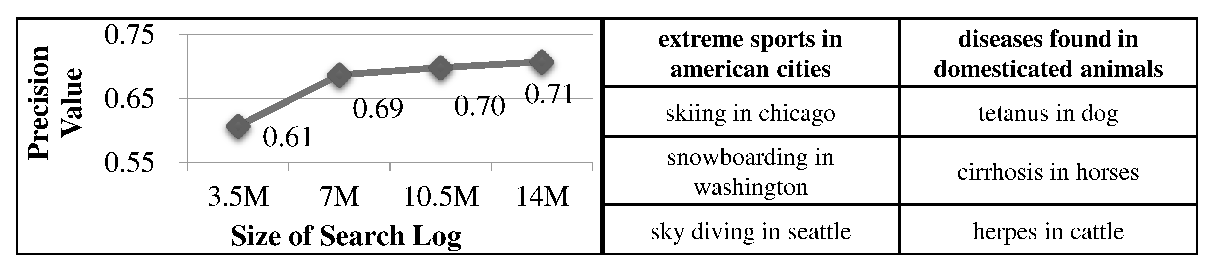
\includegraphics[width=0.9\columnwidth]{images/precision}
  \caption{Average Precision and Examples of the System} \label{fig:precision}
\end{figure}


%\begin{table}[h]
%  \centering
%  \caption{Suggestion of Two Concept-based Queries from Our System}
%  \begin{tabular}{ c|c }
%    \hline
%    \textbf{extreme sports in american cities} & \textbf{diseases found in domesticated animals}\\ \hline
%    skiing in chicago & tetanus in dog \\ \hline
%    snowboarding in washington & cirrhosis in horses \\ \hline
%    sky diving in seattle & herpes in cattle \\ \hline
%    bungee jumping in houston & cancerous growth on dog \\ \hline
%    paintball in new york & siv in cat \\ \hline
%    snowboarding los angeles & anaplasmosis in sheep \\ \hline
%    snowboarding minneapolis & mange in horses \\ \hline
%    snowboarding milwaukee & q fever in sheep \\ \hline
%  \end{tabular}
%  \centering
%  \label{tab:example}
%\end{table}

%\KZ{Maybe you can put the fig and the result table side by side in some
%way to save space?}
